\chapter{Mängder}
\label{ch:Mangder}%\nocite{Greger1971m,KTHCirkel2005rt}
\lettrine{M}{ängder är kanske} det mest grundläggande begreppet inom matematik.
Ja, kanske till och med mer grundläggande än talen.
En mängd kan beskrivas som ett matematiskt objekt som är en samling av andra
matematiska objekt.
Med andra ord, en mängd kan ses som en abstrakt påse som vi kan stoppa
matematiska saker i.
Och likt en påse som kan innehålla andra påsar kan även en mängd
innehålla andra mängder.
Det är om mängder som detta kapitel ska handla om.

I slutet av 1800-talet tillkom mängdläran till matematiken 
\cite{Kline1990mtf3}.
Äran för denna upptäckt tilldelas Georg Cantor (1845--1918).
Cantor är också utan tvekan den som bidragit mest till utvecklingen av
mängdläran.
Under sin livstid gjorde han en uttömmande utforskning av mängder och gav
häpnadsväckande resultat.
Cantor fokuserade sina studier mot oändliga mängder och han fann bland annat
att det finns fler än en oändlighet.
Heltalen och de reella talen (\cref{ch:Heltalen,ch:Reella}) är båda oändligt 
många, men Cantor visade att de reella talen var fler än de hela talen.
Han fann följaktligen att det fanns olika stora oändligheter.
Faktum är att Cantor fann att det finns oändligt många olika stora 
oändligheter.

År 1877 ställde Cantor upp sin, inom matematiken, välkända hypotes kallad
\emph{kontinuumhypotesen}\footnote{\emph{Eng.} continuum hypothesis.}.
\index{kontinuumhypotesen}\index{Cantors 
kontinuumhypotes|see{kontinuumhypotesen}}
Denna hypotes, eller förmodan, säger följande:
\begin{conjecture}[Kontinuumhypotesen]\label{Kontinuumhypotesen}
  Det finns ingen mängd vars kardinalitet är strikt mellan dem för heltalen
  och de reella talen.
\end{conjecture}
Med andra ord, det finns ingen oändlighet större än antalet heltal men mindre
än antalet reella tal.
Det är ett tomrum däremellan, alltså inget kontinuum.

Cantor kunde dock aldrig bevisa sin hypotes och faktum är att den fortfarande 
står obevisad, ingen har kunnat visa om den är sann eller falsk.
År 1963 bevisade dock Paul Cohen (1934--) med hjälp av ett resultat från 1940 
av Kurt Gödel (1906--1978) att Cantors kontinuumhypotes inte går att bevisa 
eller motbevisa inom mängdläran själv.
Det krävs nya axiom för att kunna bevisa eller motbevisa den.
Michael Rathjen (University of Leeds) höll en föreläsning vid ett kollokvium 
i Stockholm den 15 oktober 2014~\cite{smcrathjen} där han beskrev de senaste 
årens framsteg mot att finna godtagbara axiom som kan leda till att 
kontinuumhypotesen kan bevisas eller motbevisas.
Problemet här är att axiom som antas måste vara så \enquote{små} som möjligt.  
Vi vill begränsa de utsagor vi antar och istället härleda så mycket som 
möjligt.
Kontinuumhypotesen i sig är alldeles \enquote{för stor} för att vi ska kunna 
anta den som ett axiom, den är inte självklart sann som ett axiom måste vara.
Detta kommer att klarna för oss när vi strax tittar på axiomen för mängdläran.


%%%%%%%%%%%%%%%%%%%%%%%%%%%%%%%%%%%%%%%%%%%%
% ZERMELO-FRAENKELS
%%%%%%%%%%%%%%%%%%%%%%%%%%%%%%%%%%%%%%%%%%%%
\section{Zermelo--Fraenkels axiom för mängdläran}
\label{sec:Zermelo-Fraekel}
Cantor började sitt utforskande av mängdläran med en mycket enkel definition av 
vad en mängd är~\cite{Kline1990mtf3}.
Den definition som användes var följande:
\begin{definition}[Cantors mängdbegrepp]\label{CantorMangd}
  En \emph{mängd} är en samling av objekt.
  Objekt som \emph{tillhör} mängden sägs vara \emph{element} i mängden.
\end{definition}

\subsection{Russells paradox}
\label{sec:RusselsParadox}
\dots


%%%%%%%%%%%%%%%%%%%%%%%%%%%%%%%%%%%%%%%%%%%%
% BEGREPPET MÄNGD
%%%%%%%%%%%%%%%%%%%%%%%%%%%%%%%%%%%%%%%%%%%%
\section{Cantors mängdlära}

Det är nu dags att vi utforskar mängdbegreppet lite mer.
Även om Cantors definition av mängd inte längre används inom formell matematik 
är den tillräcklig för att introducera mängder och det är intressant att se 
utvecklingen.
Idag har Cantors definition ersatts av en uppsättning axiom för mängdläran,
kallade Zermelo--Fraenkels axiom efter matematikerna Ernst Zermelo (1871--1953)
och Abraham Fraenkel (1891--1965).
Den historiska utvecklingen av mängdbegreppet illustrerar väl vikten av 
formuleringarna hos de matematiska definitionerna.
Vår behandling av mängdbegreppet börjar därför med Cantors definition av mängd, 
följt av de problem som uppstår med den och slutligen ger vi Zermelo--Fraenkels 
definition.

\begin{definition}[Cantors 
  mängdbegrepp]\label{CantorMangd}\index{mängd}\index{element}
  En \emph{mängd} är en samling av objekt.
  Objekt som \emph{tillhör} mängden sägs vara \emph{element} i mängden.
\end{definition}
En mängd kan ibland också kallas för \emph{samling}.

En mängd anses vara bestämd, eller \emph{väldefinierad}, endast om man för
varje objekt kan avgöra om det ingår i mängden eller inte.
Vi säger att ett objekt \emph{tillhör} eller \emph{ej tillhör} en mängd.
Om \(M\) är en mängd och \(x\) är ett element i \(M\), då skriver vi detta som
\(x\in M\).
För ett objekt \(y\) som ej tillhör mängden \(M\) skriver vi \(y\notin M\).

Om vi vill beskriva en mängd kan vi gå tillväga på olika sätt.
Vi kan lista mängdens alla element och på så vis säga precis vad som utgör
mängden.
Detta kan bli problematiskt för mycket stora mängder, vi kan därför nöja oss
med en exakt beskrivning av vilka element som tillhör mängden.
\begin{example}\label{ExEnkelMangd}
  Låt \(M\) vara en mängd innehållandes elementen \(A,B\) och \(C\).
  Då skriver vi detta som \(M=\{A,B,C\}\).
\end{example}
\begin{example}
  Låt \(N\) vara mängden av alla namn kortare än fem bokstäver.
  Vi kan då skriva \[N=\{\text{alla namn kortare än fem bokstäver}\}\] eller
  \[N=\{n\colon n\text{ är ett namn kortare än fem bokstäver}\}\] som utläses
  \(N\) är mängden av alla \(n\) sådana att \(n\) är ett namn kortare än fem
  bokstäver.
  Denna mängd är väldefinierad för vi kan enkelt avgöra om ett element
  tillhör mängden eller inte.
  Om ett objekt ej är ett namn, då tillhör det heller inte mängden.
  Om ett objekt är ett namn och om det också är kortare än fem bokstäver
  tillhör det mängden, annars inte.
\end{example}
\begin{example}\label{ExTommaMangden}
  Den tomma mängden som inte har några element betecknas med \(\emptyset\).
  Vi har följaktligen att \(\emptyset=\{\}\).
\end{example}

Vi kan illustrera mängder som ringar som omsluter elementen som tillhör
mängden.
En sådan illustration kallas för Venndiagram, namngivet efter den brittiske 
logikern och filosofen John Venn (1834--1923).
Ett exempel på Venndiagram med två mängder kan ses i \cref{fig:Disjunkt}.
\begin{figure}
  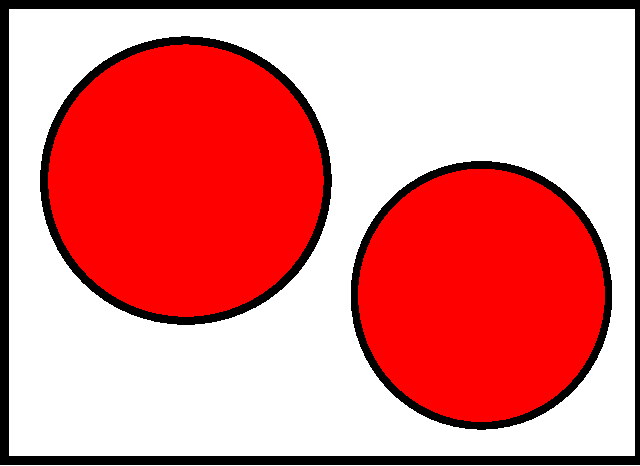
\includegraphics[width=4cm]{figs/disjoint.pdf}
  \caption{%
    Två mängder.
    Bild:~\cite{Wikipedia2013Set}.
  }\label{fig:Disjunkt}
\end{figure}

Vi kan nu skapa mängder och tala om vilka element de innehåller, men hur kan vi
jämföra två mängder?
Hur vet vi om två mängder är lika?
\begin{definition}\label{def:Mangdlikhet}\index{mängd!likhet}\index{likhet}
  Vi säger att två mängder \(A\) och \(B\) är \emph{lika} om varje element i
  \(A\) även tillhör \(B\) och varje element i \(B\) även tillhör \(A\).
  Om \(A\) och \(B\) är lika skriver vi \(A=B\), annars skriver vi \(A\neq
  B\).
\end{definition}
\begin{exercise}\label{XrcLikhetMangd}
  Undersök vad detta innebär, vilka mängder är egentligen lika?
  Är \(\{1,2,3\}\) lika med \(\{1,1,3,3,2,3,2,1\}\)?
\end{exercise}
\begin{exercise}
  I inledning sades att en mängd kan innehålla andra mängder.
  En mängd \(X\) som tillhör en mängd \(M\) är då ett element som alla andra i
  mängden \(M\).
  Om \(X=\{1,2\}\) och \(M=\{X, 2, 3\}=\{\{1,2\},2,3\}\), vilka av följande
  utsagor är sanna och vilka är falska: 
  \(1\in M\), \(2\in M\) och \(3\in M\) samt \(\{1\}\in M\),
  \(\{2\}\in M\) och \(\{1,2\}\in M\).
\end{exercise}
\begin{exercise}\label{XrcBeskrivaTommaMangden}
  På hur många sätt kan man egentligen matematiskt beskriva den tomma
  mängden?
\end{exercise}

Vi fortsätter med ett annat viktigt begrepp, disjunktionen.
\begin{definition}\label{def:Disjunkt}\index{disjunkt}
  Två mängder \(A\) och \(B\) sägs vara \emph{disjunkta} om varje element i
  \(A\) ej är ett element i \(B\).
\end{definition}
\begin{exercise}
  Om \(A\) och \(B\) är mängder, betyder det samma sak att \(A\neq B\) som
  att \(A\) och \(B\) är disjunkta?
\end{exercise}
Mängderna i \cref{fig:Disjunkt} är disjunkta medan mängderna 
i \cref{fig:IckeDisjunkt} inte är det.
\begin{figure}
  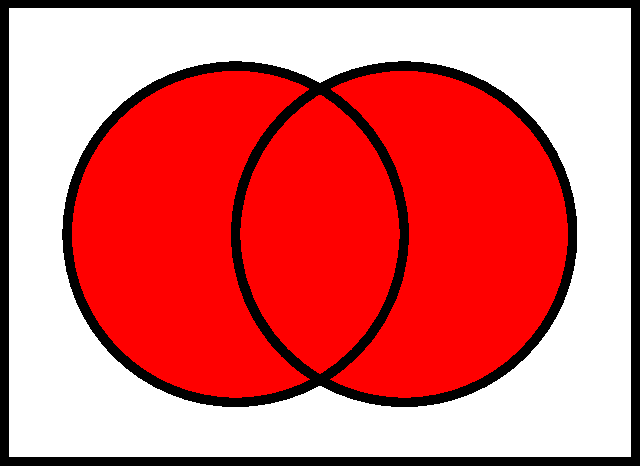
\includegraphics[width=4cm]{figs/union.pdf}
  \caption{%
    Två icke disjunkta mängder.
    Bild:~\cite{Wikipedia2013Set}.
  }\label{fig:IckeDisjunkt}
\end{figure}


%%%%%%%%%%%%%%%%%%%%%%%%%%%%%%%%%%%%%%%%%%%%
% OPERATIONER PÅ MÄNGDER
%%%%%%%%%%%%%%%%%%%%%%%%%%%%%%%%%%%%%%%%%%%%
\section{Operationer på mängder}
\label{sec:Mangdoperationer}
Efter att ha tittat på vad en mängd är och hur vi kan avgöra om
två mängder är lika ska vi nu titta på hur vi kan skapa nya mängder genom att
kombinera mängder som vi redan har.

\begin{definition}\label{def:Union}\index{union}
  Låt \(A\) och \(B\) vara mängder.
  Vi låter mängden \(A\cup B\) av alla element i \(A\) och alla element i
  \(B\) kallas för \emph{unionen} av \(A\) och \(B\).
  Det vill säga, \(A\cup B = \{x\colon x\in A\tor x\in B\}\).
\end{definition}
Detta illustreras med ett Venndiagram i \cref{fig:Union}.
\begin{figure}
  % XXX typeset set union figure with tex
  % XXX use eps format for figure
  \subfloat[Mängden \(A\).]{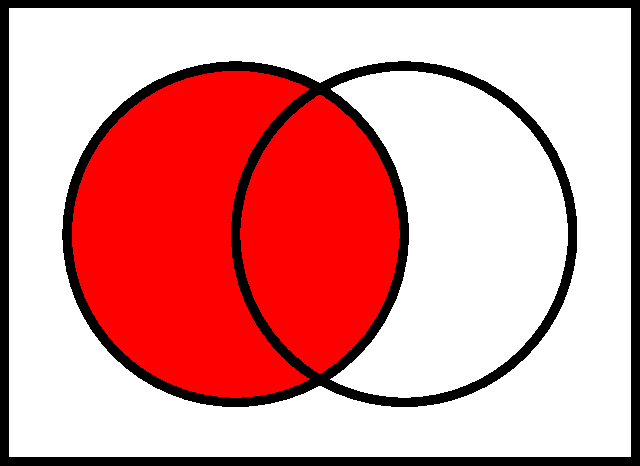
\includegraphics[width=4cm]{figs/A.pdf}}
  \subfloat[Mängden \(B\).]{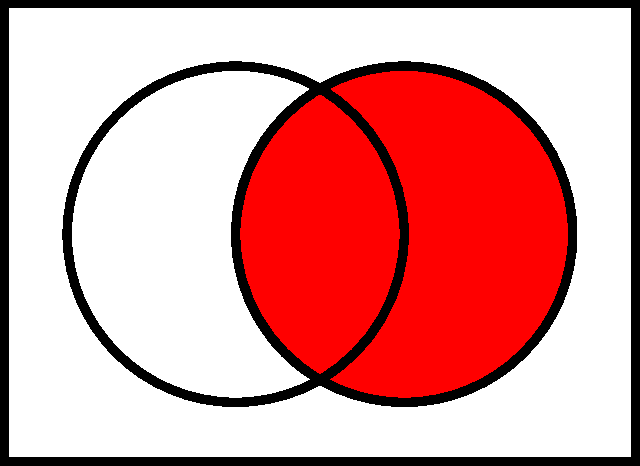
\includegraphics[width=4cm]{figs/B.pdf}}
  \subfloat[Mängden \(A\cup B\).]{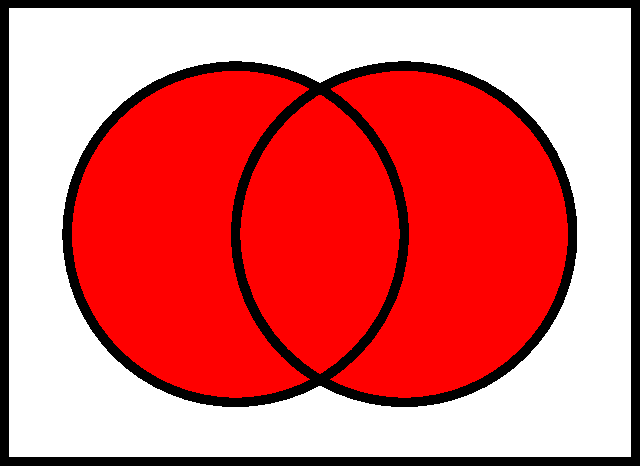
\includegraphics[width=4cm]{figs/union.pdf}}
  \caption{%
    Unionen av två mängder.
    Bild:~\cite{Wikipedia2013Set}.
  }\label{fig:Union}
\end{figure}

\begin{exercise}
  Utforska unionsoperationen, finns det några intressanta resultat om detta?
\end{exercise}

\begin{definition}\label{def:Snitt}\index{snitt}
  Låt \(A\) och \(B\) vara mängder.
  Vi låter mängden \(A\cap B\) av alla element i \(A\) som också tillhör
  \(B\) kallas för \emph{snittet} mellan \(A\) och \(B\).
  Det vill säga, \(A\cap B = \{x\colon x\in A\tand x\in B\}\).
\end{definition}
Begreppet snitt illustreras med ett Venndiagram i \cref{fig:Snitt}.
\begin{figure}
  % XXX typeset set intersection figure with tex
  % XXX use eps format for figure
  \subfloat[Mängden \(A\).]{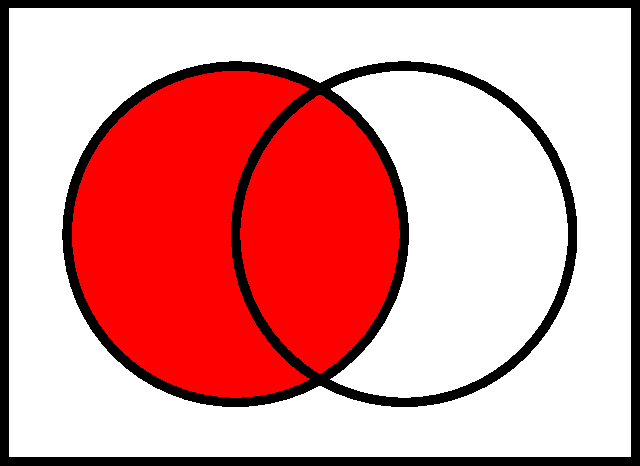
\includegraphics[width=4cm]{figs/A.pdf}}
  \subfloat[Mängden \(B\).]{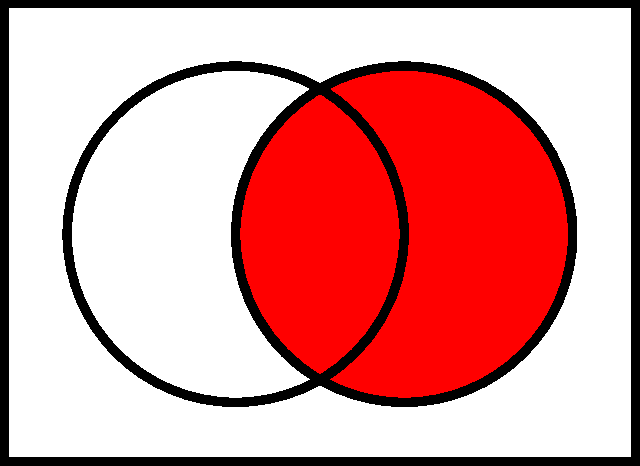
\includegraphics[width=4cm]{figs/B.pdf}}
  \subfloat[Mängden \(A\cap B\).]{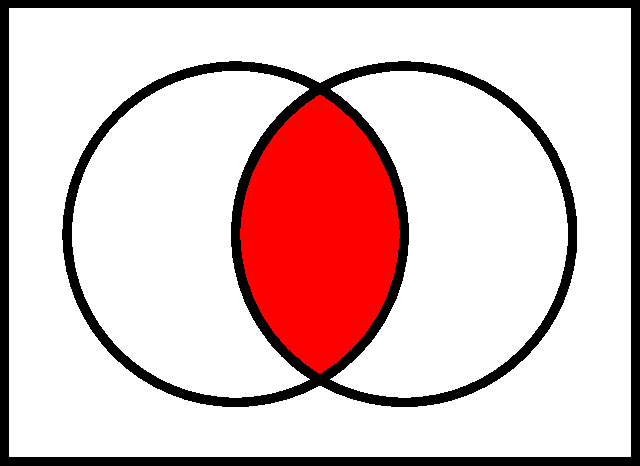
\includegraphics[width=4cm]{figs/intersection.pdf}}
  \caption{%
    Snittet av två mängder.
    Bild:~\cite{Wikipedia2013Set}.
  }\label{fig:Snitt}
\end{figure}

\begin{exercise}
  Utforska snittoperationen, finns det några intressanta resultat om detta?
\end{exercise}

\begin{exercise}
  Hur förhåller sig unions- och snittoperationerna?
  Exempelvis, spelar det någon roll om vi tar snittet av två unioner eller om 
  vi tar unionen av två snitt?
\end{exercise}

\begin{definition}\label{def:Mangddifferens}\index{differens}\index{mängd!differens}
  Låt \(A\) och \(B\) vara mängder.
  Vi låter mängden \(A\setminus B\) av alla element i \(A\) som inte tillhör
  \(B\) kallas för \emph{differensen} mellan \(A\) och \(B\).
  Det vill säga, \(A\setminus B = \{x\colon x\in A\tand x\notin B\}\).
\end{definition}
En illustration över mängderna \(A\), \(B\) och differensen \(A\setminus B\) 
ges i \cref{fig:Differens}.
\begin{figure}
  % XXX typeset set difference figure with tex
  % XXX use eps format for figure
  \subfloat[Mängden \(A\).]{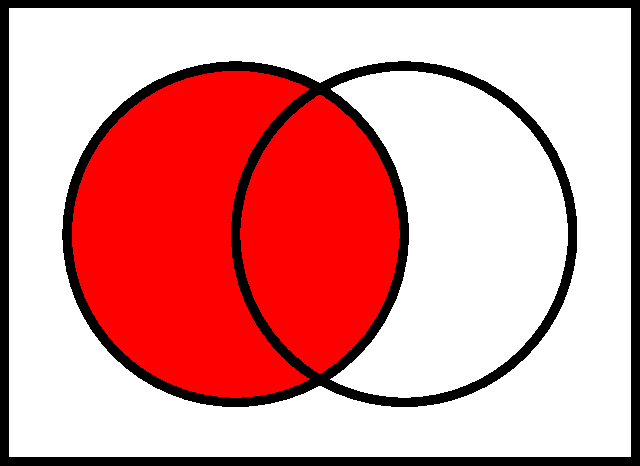
\includegraphics[width=4cm]{figs/A.pdf}}
  \subfloat[Mängden \(B\).]{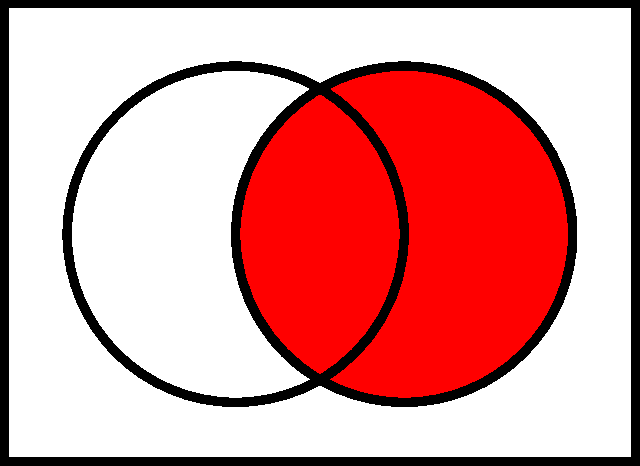
\includegraphics[width=4cm]{figs/B.pdf}}
  \subfloat[Mängden \(A\setminus B\).]{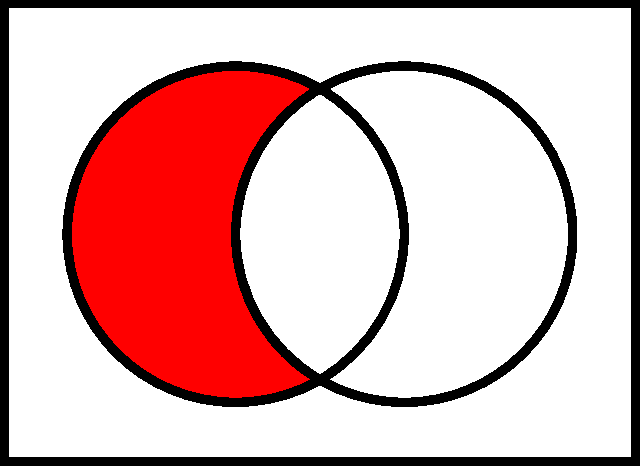
\includegraphics[width=4cm]{figs/A_setminus_B.pdf}}
  \caption{%
    Differensen av två mängder.
    Bild:~\cite{Wikipedia2013Set}.
  }\label{fig:Differens}
\end{figure}

\begin{exercise}
  Blir det någon skillnad om vi istället definierar differensen som 
  \(A\setminus B = \{x\colon x\notin A\tand x\in B\}\)?
\end{exercise}
\begin{exercise}
  Finns det några intressanta resultat om differensen?
  Hur förhåller sig denna operation gentemot operationerna union och snitt?
\end{exercise}

\begin{definition}\label{def:KartesiskProdukt}\index{kartesisk produkt}
  Låt \(M\) och \(N\) vara mängder.
  Mängden \(\{(m,n)\colon m\in M\tand n\in N\}\) av alla ordnade par med första
  element i \(M\) och andra element i \(N\) 
  kallas för den \emph{kartesiska produkten} av \(M\) och \(N\) och skrivs
  \(M\times N\).
\end{definition}
Namnet kartesisk produkt kommer från den franske matematikern och filosofen
René Descartes (1596--1650) vars latinska namn var Renatus Cartesius.
Descartes matematiska studier gav upphov till denna typ av begrepp och därför
är den kartesiska produkten i efterhand uppkallad efter honom.

\begin{exercise}\label{xrc:Kortlek}
  Låt \(V\) vara mängden av alla valörer i en kortlek, det vill säga
  \(V=\{2,3,4,5,6,7,8,9,10,\text{knekt},\text{dam},\text{kung},\text{ess}\}\).
  Låt också \(F\) vara mängden av färger i en kortlek, det vill säga
  \(F=\{\spadesuit,\clubsuit,\heartsuit,\diamondsuit\}\).
  Vad blir \(F\times V\) och vad skulle denna mängd kunna användas för att
  representera?
\end{exercise}


%%%%%%%%%%%%%%%%%%%%%%%%%%%%%%%%%%%%%%%%%%%%
% DELMÄNGDER
%%%%%%%%%%%%%%%%%%%%%%%%%%%%%%%%%%%%%%%%%%%%
\section{Delmängder}
\label{sec:Delmangder}
Härnäst ska vi titta på delar av mängder, eller mängder vars
element utgör en del av de element som finns i en annan mängd.
Detta är intressant för att det är inte alltid som vi är intresserade av hela
mängden, det är inte heller alltid som vi bara är intresserade av enbart ett
element.
Ibland kan det vara intressantare att titta på en del av elementen i en mängd,
och från dessa skapa en ny mängd.
Vi ger därför följande definition.

\begin{definition}\label{def:Delmangd}\index{delmängd}
  Låt \(A\) och \(B\) vara mängder.
  Vi säger att \(A\) är en \emph{delmängd} av \(B\) om varje element i \(A\)
  även tillhör \(B\).
  Vi skriver detta som \(A\subseteq B\) och utläser det som att \emph{\(A\)
  är inkluderad i \(B\)}.
  Vi kan likvärdigt skriva \(B\supseteq A\) och utläser detta som att
  \emph{\(B\) inkluderar \(A\)}.
  Om dessutom \(A\neq B\) är \(A\) en \emph{äkta} eller \emph{proper
  delmängd} av \(B\) och detta skrivs \(A\subset B\) respektive
  \(B\supset A\).
\end{definition}
I \cref{fig:Delmangd} illustreras begreppet genom ett Venndiagram.
\begin{figure}
  % XXX typeset set complement figure with tex
  % XXX use eps format for figure
  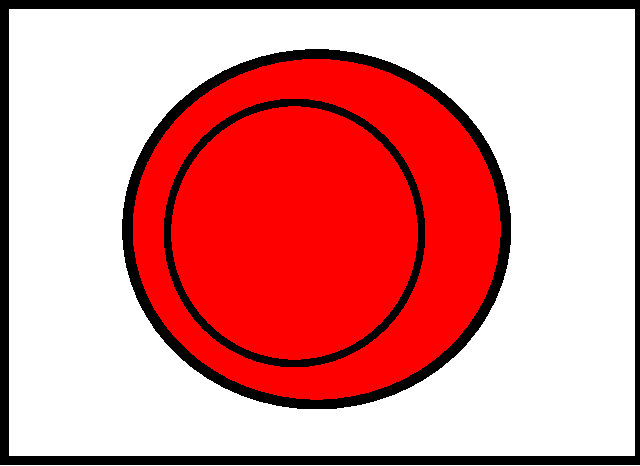
\includegraphics[width=4cm]{figs/subset.pdf}
  \caption{%
    Två mängder, där den ena är inkluderad av den andre.
    Bild:~\cite{Wikipedia2013Set}.
  }\label{fig:Delmangd}
\end{figure}

\begin{exercise}
  Vad skulle det innebära om \(A\) är en delmängd av \(B\) och \(B\) är en
  delmängd av \(A\), det vill säga \(A\subseteq B\) och \(B\subseteq A\)?
  Är detta ens möjligt?
  Det är faktiskt så att det är en vanlig bevismetod inom matematiken att
  först visa \(A\subseteq B\) och sedan visa \(B\subseteq A\).
\end{exercise}

Vi fortsätter med en annan definition med koppling till delmängdsbegreppet.
\begin{definition}\label{def:Komplement}\index{komplement}
  Låt \(A\) vara en delmängd till mängden \(B\).
  Vi kallar mängden \(A^\complement = B\setminus A\) för \emph{komplementet}
  till \(A\) i mängden \(B\).
\end{definition}
Begreppet illustreras med ett Venndiagram i \cref{fig:Komplement}.
\begin{figure}
  % XXX typeset set complement figure with tex
  % XXX use eps format for figure
  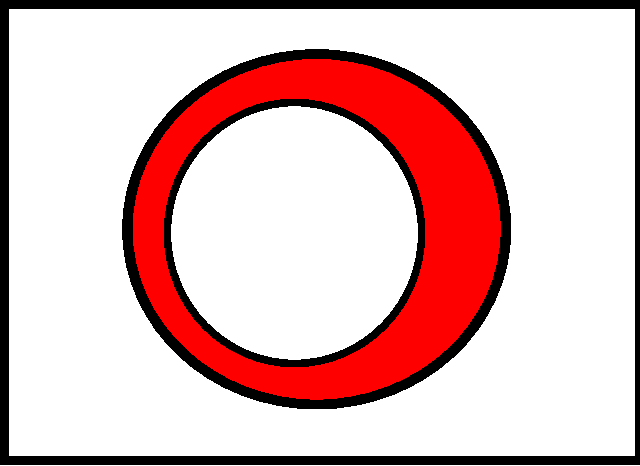
\includegraphics[width=4cm]{figs/complement.pdf}
  \caption{%
    Komplementet till en delmängd.
    Bild:~\cite{Wikipedia2013Set}.
  }\label{fig:Komplement}
\end{figure}

\begin{exercise}
  Vad är det för skillnad mellan begreppen komplement och differens?
\end{exercise}

\begin{example}
  Låt \(M=\{1,2,3\}\) och \(A=\{1,2\}\) vara två mängder.
  Då har vi att \(A\subseteq M\), det vill säga \(A\) är en delmängd till
  \(M\), och faktiskt \(A\subset M\), det vill säga \(A\) är en äkta delmängd
  till \(M\).
  Vi har dessutom att komplementet till \(A\) är \(A^\complement =
  M\setminus A = \{3\}\).
\end{example}

Nu när vi har delmängder till en mängd \(M\), då kan det vara skönt att ha ett
enkelt notationssätt för mängden av alla delmängder till \(M\).
Denna mängd som innehåller alla delmängder till \(M\) som element kallas
\emph{potensmängd} och definieras härnäst.
\begin{definition}\label{def:Potensmangd}\index{potensmängd}
  Låt \(M\) vara en mängd.
  Vi kallar mängden av alla delmängder till \(M\) för \emph{potensmängden}
  av \(M\).
  Vi betecknar potensmängden till \(M\) som \(\powerset(M)\).
\end{definition}
\begin{exercise}
  Undersök hur potensmängden av en mängd \(M\) förhåller sig till mängden
  \(M\) själv.
\end{exercise}


%%%%%%%%%%%%%%%%%%%%%%%%%%%%%%%%%%%%%%%%%%%%
% RELATIONER
%%%%%%%%%%%%%%%%%%%%%%%%%%%%%%%%%%%%%%%%%%%%
\section{Relationer}\label{Relationer}

Vi ska nu titta på hur vi kan upprätta relationer mellan
elementen i en mängd.
I tidigare avsnitt har vi redan stött på en relation -- likheten mellan två
mängder.

\begin{definition}\label{def:BinarRelation}\index{relation}\index{binär 
    relation}
  En \emph{binär relation} \(R\) på en mängd \(M\) är en delmängd till den
  kartesiska produkten \(M\times M\).
  Om \((x,y)\in M\times M\) tillhör \(R\) skriver vi \(x\mathop R y\) som 
  utläses
  \emph{\(x\) är relaterat till \(y\) via \(R\)}.
\end{definition}

\begin{remark}\label{RelationDelmangdTillKartesiskProdukt}
  Mängden \(R\) är följaktligen en delmängd till den kartesiska produkten
  \(M\times M\).
\end{remark}

Enligt denna definition skulle likhetsrelationen mellan mängder vara en
relation på mängden av alla mängder och två mängder i denna mängd är relaterade
om de uppfyller kraven i \cref{def:Mangdlikhet}.
Vi ska titta på ett mindre abstrakt exempel.
\begin{example}
  Låt \(S\) vara mängden av alla personer som är skrivna på en adress i
  Sverige.
  Två personer \(p\in S\) och \(q\in S\) är relaterade via relationen \(G\)
  om de bor på samma gata.
  Om \(p\) bor på \enquote{Gatuvägen 1, 123\,45 Kommunen} och \(q\) bor på
  \enquote{Gatuvägen 3, 123\,45 Kommunen}, då gäller att \(p\mathop G q\) 
  eftersom att båda bor på \enquote{Gatuvägen}.

  Vi kan då också beskriva \(G\) på följande vis.
  Låt \(V_i\) vara mängden av alla personer som är skriva på någon väg \(i\).
  Då är \(G\) unionen av \(V_i\times V_i\) för alla vägar \(i\) i Sverige.
\end{example}

\begin{exercise}
  Använd mängderna som definieras i \cref{xrc:Kortlek} och definiera en
  relation för någon dessa.
  Inspiration: Du kan utgå från ditt favoritkortspel och definiera en eller
  flera lämpliga relationer mellan kort eller mängder av kort.
\end{exercise}


%%%%%%%%%%%%%%%%%%%%%%%%%%%%%%%%%%%%%%%%%%%%
% EKVIVALENSKLASS
%%%%%%%%%%%%%%%%%%%%%%%%%%%%%%%%%%%%%%%%%%%%
\subsection{Ekvivalensrelation och ekvivalensklass}
Vi ska nu titta på en speciell typ av relation -- ekvivalensrelationen.
Ekvivalensrelationen har en särskild struktur för hur element är relaterade
till varandra.
Den har sitt namn från att den påminner om likhetsbegreppet som vi tagit upp
tidigare.

\begin{definition}\label{def:Ekvivalensrelation}\index{ekvivalensrelation}\index{relation!ekvivalensrelation}
  En binär relation \(R\) på en mängd \(M\) som uppfyller att
  \begin{enumerate}
    \item för alla \(x\in M\) gäller att \(x\mathop R x\) (reflexivitet),
    \item för alla \(x,y\in M\) gäller att om \(x\mathop R y\) då gäller även
      \(y\mathop R x\) (symmetri),
    \item för alla \(x,y,z\in M\) gäller att om \(x\mathop R y\) och \(y\mathop 
      R z\)
      då gäller även att \(x\mathop R z\) (transitivitet),
  \end{enumerate}
  kallas för \emph{ekvivalensrelation}.
\end{definition}
\begin{exercise}
  Undersök vilka relationer du känner till som är reflexiva, symmetriska och
  transitiva, och följaktligen är ekvivalensrelationer.
\end{exercise}

En ekvivalensrelation \emph{partitionerar} en mängd \(M\) i disjunkta
delmängder kallade partitioner.
Dessa partitioner utgörs av något som brukar
kallas för ekvivalensklasser. %, som är disjunkta delmängder av mängden \(M\).
\begin{definition}\label{def:Ekvivalensklass}\index{ekvivalensklass}\index{ekvivalensrelation!ekvivalensklass}
  Låt \(R\) vara en ekvivalensrelation definierad på mängden \(M\).
  Om \(a\) är ett element i \(M\), då kallar vi mängden
  \(\{x\in M\colon x\mathop R a\}\) för \emph{ekvivalensklassen} för \(a\) och 
  betecknar denna som \([a]_R\), elementet \(a\) sägs vara en 
  \emph{representant} för ekvivalensklassen.
\end{definition}
Om det är klart under vilken relation ekvivalensklassen gäller räcker det med
att skriva \([a]\) istället för \([a]_R\).

På samma sätt som att det går att skapa en partition genom att införa en
ekvivalensrelation på mängden går det också att skapa en ekvivalensrelation på
mängden genom att partitionera den.

\begin{example}
  Låt \(F\) vara mängden av alla fåglar.
  Vi inför en relation \(A\) där två fåglar \(x\) och \(y\) är relaterade via
  \(A\) om de tillhör samma fågelart.
  Är detta en ekvivalensrelation?
  Om \(x\) är en berguv (\emph{Bubo bubo}), då måste \(x\mathop A x\) eftersom 
  att \(x\) tillhör samma fågelart som sig själv.
  Således är relationen reflexiv.
  Om \(x\) är en berguv och om \(x\mathop A y\), då måste även \(y\) vara en 
  berguv och följaktligen \(y\mathop A x\).
  Relationen är därför symmetrisk.
  Om \(x\) är en berguv och \(x\mathop A y\), då måste \(y\) vara en berguv.
  Om dessutom \(y\mathop A z\) måste \(z\) också vara en berguv.
  Eftersom både \(x\) och \(z\) är berguvar gäller att \(x\mathop A z\).
  Då är relationen transitiv.
  Relationen uppfyller kraven för en ekvivalensrelation och måste
  därför vara en ekvivalensrelation.

  Eftersom att relationen \(A\) är en ekvivalensrelation innebär det att den
  partitionerar mängden \(F\) av alla fåglar.
  Varje partition, eller ekvivalensklass, är en mängd av alla fåglar inom
  samma art.
  Exempelvis är mängden av alla berguvar en ekvivalensklass.
\end{example}

\begin{figure}
  % XXX typeset set partition figure with tex
  % XXX use eps format for figure
  
\includegraphics[width=5cm]{figs/set_partition.pdf}
  \caption{%
    En mängd (hela cirkeln) som är partitionerad i sex delmängder.
    Varje delmängd (färg) representerar en ekvivalensklass.
  }\label{fig:setPartition}
\end{figure}

Mängden av alla ekvivalensklasser hos \(M\) under relationen \(\sim\)
brukar betecknas \(M/\!\sim\) och kallas för \emph{kvotmängden av \(M\)
och \(\sim\)}\index{kvotmängd}.
Om \(m\) är ett element i \(M\), då är \([m]_\sim\) ett element i kvotmängden
\(M/\!\sim\).


%%%%%%%%%%%%%%%%%%%%%%%%%%%%%%%%%%%%%%%%%%%%
% AVBILDNINGAR
%%%%%%%%%%%%%%%%%%%%%%%%%%%%%%%%%%%%%%%%%%%%
\section{Avbildningar}
Vi ska nu införa ett annat väldigt centralt begrepp inom matematiken.
Vi ska titta på avbildningar, eller funktioner som kanske är det mer kända 
namnet.
Vi börjar med att definiera vad en funktion är.

\begin{definition}\label{def:Avbildning}\index{avbildning}\index{funktion}
  Låt \(A\) och \(B\) vara mängder.
  En \emph{funktion}, eller \emph{avbildning}, \(f\colon A\to B\) tilldelar
  till varje \(a\in A\) ett välbestämt \(b\in B\).
  Vi skriver \(f(a)=b\) eller \(a\mapsto b\) och säger att \(a\)
  \emph{avbildas} på \(b\) eller att \(b\) är \emph{bilden} av \(a\).
  Mängden \(A\) sägs vara funktionens \emph{definitionsmängd} och mängden
  \(B\) sägs vara funktionens \emph{värdemängd}.
\end{definition}
\begin{remark}
  Notera att varje funktion \(f\colon A\to B\) ger en funktionsgraf \(G_f\)
  som är en delmängd till den kartesiska produkten \(A\times B\).
  Det vill säga, \(G_f = \{(a,b)\in A\times B\colon f(a)=b\}\).
  Då är \((a,b)\in G_f\) om \(f(a)=b\), eller \(a\mapsto b\).
\end{remark}
\begin{example}
  Låt \(A=\{1,2,3\}\) och \(B=\{x,y,z\}\) vara mängder.
  Vi låter \(f\colon A\to B\) vara en funktion från \(A\) till \(B\).
  Vi låter \(1\mapsto x\), \(2\mapsto z\) och \(3\mapsto y\).
  Vi har då exempelvis att \(2\) avbildas på \(f(2)=z\).
\end{example}

\begin{exercise}
  Skulle en funktion kunna ses som en relation?
\end{exercise}

I de flesta fall är det inte lämpligt att lista alla avbildningarna för
funktionen, det vill säga ge dess funktionsgraf, som vi gjorde ovan.
Istället är det bättre att ge en beskrivning av hur elementen ska avbildas.
Vi ska illustrera med två exempel.
\begin{example}
  Låt \(M\) vara mängden av alla människor i Sverige och \(P\) vara mängden
  av alla geografiska platser på jorden.
  Låt \(p\colon M\to P\) vara en avbildning från \(M\) till \(P\).
  Vi avbildar då varje människa i \(M\) på den geografiska plats i \(P\) där
  den föddes.
\end{example}
\begin{example}
  Låt \(f\colon M\to M\) vara en avbildning från mängden
  \(M=\{0,1,2,3,\ldots\}\) till sig själv, och låt \(x\) avbildas på
  \(f(x)=x+1\).
\end{example}

Vi ska nu införa en egenskap för avbildningar.
Vi vill kunna beskriva en funktion som avbildar element på ett särskilt vis.
\begin{definition}\label{def:Injektiv}\index{injektiv}
  Låt \(f\) vara en funktion från en mängd \(A\) till en mängd \(B\).
  Vi säger att \(f\) är \emph{injektiv} om för varje \(x\in A\) och \(y\in
  A\) gäller att om \(f(x)=f(y)\) då är även \(x=y\).
\end{definition}
\begin{example}\label{ex:Surjektiv}
  Låt \(A=\{1,2,3\}\) och \(B=\{a,b\}\) vara mängder samt låt \(f\) vara en
  funktion från \(A\) till \(B\).
  Vi låter \(f(1)=a\), \(f(2)=b\) och \(f(3)=b\).
  Då är \(f\) inte injektiv eftersom att \(f(2)=f(3)\) men \(2\neq 3\).
\end{example}
\begin{example}\label{ex:Injektiv}
  Låt \(A=\{1,2\}\) och \(B=\{a,b,c\}\) vara mängder samt låt \(f\) vara en
  funktion från \(A\) till \(B\).
  Vi låter \(f(1)=a\) och \(f(2)=b\).
  Då är \(f\) injektiv eftersom att det för alla element \(x\in A\) gäller
  att om \(f(x)=f(y)\) då är \(x=y\).
\end{example}

En annan injektion illustreras i \cref{fig:Injektion}.
\begin{figure}
  % XXX typeset injection figure with tex
  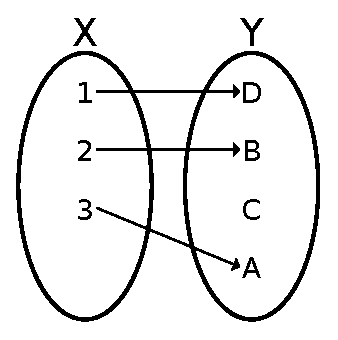
\includegraphics[width=4cm]{figs/injection.eps}
  \caption{%
    En injektiv funktion från en mängd \(X=\{1,2,3\}\) till en mängd
    \(Y=\{A,B,C,D\}\).
    Bild:~\cite{Wikipedia2013Injection}.
  }\label{fig:Injektion}
\end{figure}

Vi ska införa en till egenskap likt den ovan.
\begin{definition}\label{def:Surjektiv}\index{surjektiv}
  Låt \(f\) vara en funktion från en mängd \(A\) till en mängd \(B\).
  Vi säger att \(f\) är \emph{surjektiv} om det för varje \(b\in B\)
  existerar ett \(a\in A\) sådant att \(b=f(a)\).
\end{definition}
\begin{example}
  Funktionen \(f\) i \cref{ex:Surjektiv} är surjektiv eftersom att
  det för varje element \(y\in B\) finns ett element i \(x\in A\) sådant
  att \(f(x)=y\).
\end{example}
\begin{example}
  Funktionen \(f\) i \cref{ex:Injektiv} är ej surjektiv eftersom att
  det finns ett element i \(B\), nämligen \(c\), sådant att
  \(f(x)\neq c\) för alla \(x\in A\).
\end{example}

I \cref{fig:Surjektion} illustreras ytterligare en surjektion.
\begin{figure}
  % XXX typeset surjection figure with tex
  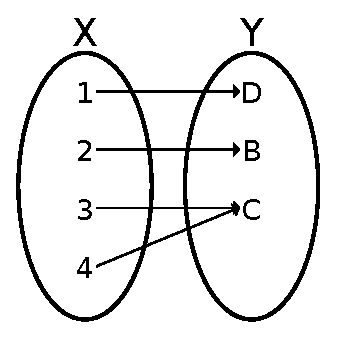
\includegraphics[width=4cm]{figs/surjection.eps}
  \caption{%
    En surjektiv funktion från en mängd \(X=\{1,2,3,4\}\) till en
    mängd \(Y=\{B,C,D\}\).
    Bild:~\cite{Wikipedia2013Injection}.
  }\label{fig:Surjektion}
\end{figure}

\begin{definition}
  En avbildning som är både injektiv och surjektiv sägs vara
  \emph{bijektiv}\index{bijektiv}.
\end{definition}
\begin{exercise}
  Vad ändra mängderna i \cref{ex:Injektiv,ex:Surjektiv} för att dessa ska vara 
  bijektiva?
\end{exercise}

En bijektiv funktion illustreras i \cref{fig:Bijektion}.
\begin{figure}
  % XXX typeset bijection figure with tex
  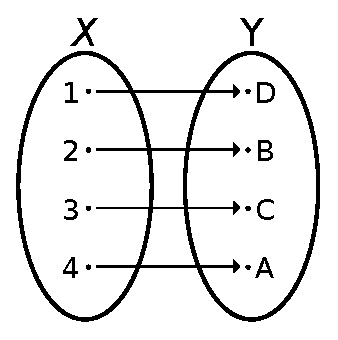
\includegraphics[width=4cm]{figs/bijection.eps}
  \caption{%
    En bijektiv funktion från en mängd \(X=\{1,2,3,4\}\) till en
    mängd \(Y=\{A,B,C,D\}\).
    Bild:~\cite{Wikipedia2013Injection}.
  }\label{fig:Bijektion}
\end{figure}


%%%%%%%%%%%%%%%%%%%%%%%%%%%%%%%%%%%
% KARDINALITET
%%%%%%%%%%%%%%%%%%%%%%%%%%%%%%%%%%%
\section{Kardinalitet}
Vi kan avgöra om två mängder är lika genom att undersöka om alla
element finns med i båda mängderna, om de gör det så är mängderna lika.
Om det däremot saknas element kan vi i nuläget inte säga mycket mer än att
mängderna är olika.
Det kan dock vara intressant att kunna se hur två disjunkta mängder förhåller
sig till varandra.
Till exempel genom att bestämma hur stora de är.

När vi avgör hur stort någonting är, med avseende på antal, brukar vi räkna
antalet objekt.
Om vi exempelvis skulle avgöra hur många personer vi ser just nu börjar vi med
att peka på en person och säga \emph{ett}, peka på en annan person och säga
\emph{två}, och så vidare tills att vi har pekat på samtliga personer vi kan se.
Det vi egentligen gör när vi räknar på detta vis är att upprätta en avbildning
från talen \(1,2,3,\ldots\) till objekten vi räknar.
Vi kan utifrån denna idé definiera storleken för mängder, kallad en mängds
\emph{kardinalitet}, på följande vis.
\begin{definition}\label{def:Kardinalitet}\index{kardinalitet}
  Om \(A\) och \(B\) är mängder säger vi att de har samma \emph{kardinalitet}
  om det finns en bijektiv avbildning mellan \(A\) och \(B\).
  Vi skriver då att \(\card A = \card B\) eller \(|A| = |B|\).
  Om \(A\) har samma kardinalitet som mängden \(\{1,2,3,\ldots,n\}\) för
  något naturligt tal \(n\) skriver vi \(|A| = n\).
  Den tomma mängden \(\emptyset\) har kardinalitet \(|\emptyset| = 0\).
\end{definition}

\begin{example}
  Mängderna \(M=\{a,b,c\}\) och \(N=\{1,2,3\}\) har samma kardinalitet,
  nämligen \(3\).
  Detta eftersom att avbildningen \(f\colon M\to N\) sådan att \(f(a)=1\),
  \(f(b)=2\) och \(f(c)=3\) är bijektiv.
\end{example}

Anledningen till att vi definierar kardinalitet på detta vis är för att det är 
detta vi faktiskt gör när vi räknar, vi ställer upp en bijektion till en 
delmängd av de naturliga talen \(\N\).
Denna formulering är dock mer generell då vi inte låser oss till de naturliga 
talen.
Detta är viktigt då antalet element i mängden blir oändligt, men trots att de 
är oändligt stora vill vi fortfarande kunna jämföra dem.
Det var just detta som Cantor gjorde, och vi har redan i inledningen nämnt
några av de resultat som han kom fram till.
